\newpage
\sect{Live-Streaming auf Youtube}

{\vspace{0.2cm}}
\begin{center}
  \textbf{Hierfür klickt hierfür auf \quote{Livestream starten } rechts oben.} \\
  \textbf{(Dies setzt voraus das OBS mit Youtube verbunden ist.)} \\
  {\vspace{0.3cm}}
  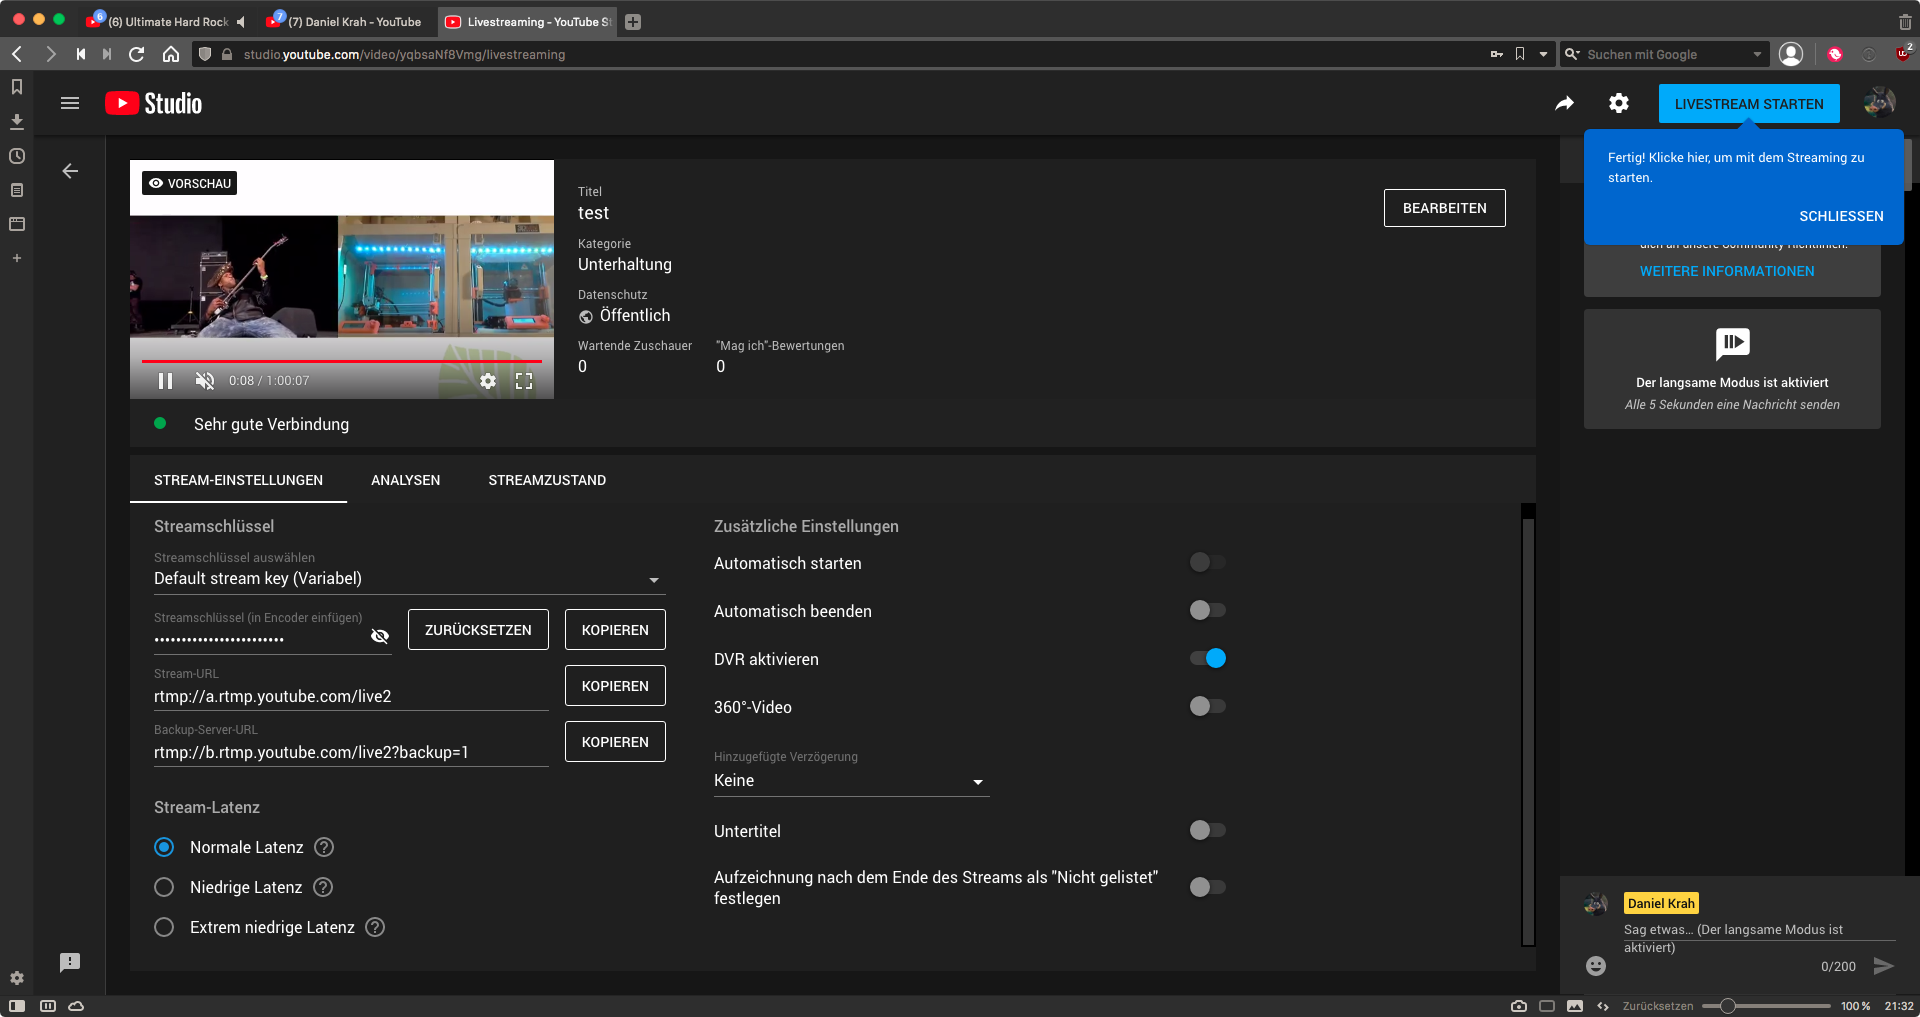
\includegraphics[width=0.7\textwidth]{./pictures/OBSYOutubeConnected.png}
\end{center}



% {\vspace{-0.6cm}}
\begin{center}
  \textbf{Während der Stream started sieht man einen rotierenden Kreis in der Vorschau.} \\
  {\vspace{0.3cm}}
  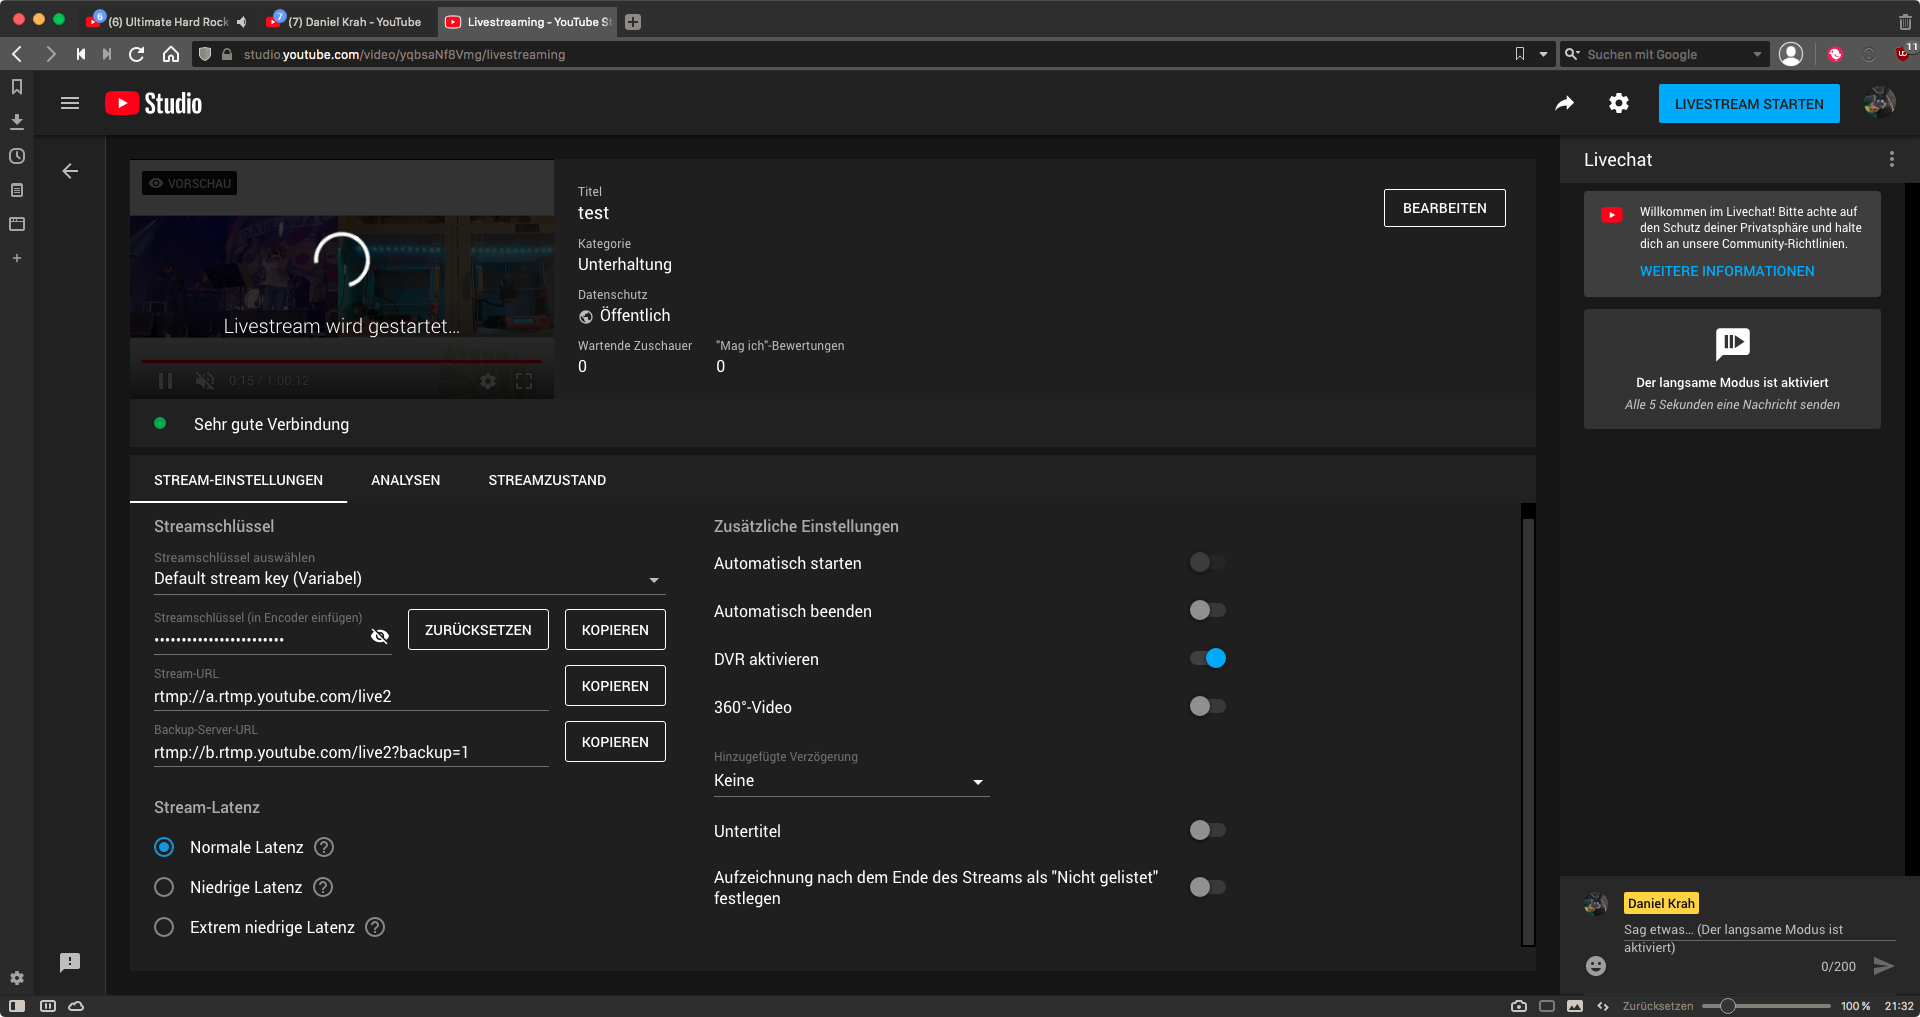
\includegraphics[width=0.7\textwidth]{./pictures/OBSYOutubeConnected-START.png}
\end{center}

\newpage
% {\vspace{-0.6cm}}
\begin{center}
  \textbf{Einen Live-Stream kann man auch über Streamlabs OBS starten.} \\
  {\vspace{0.3cm}}
  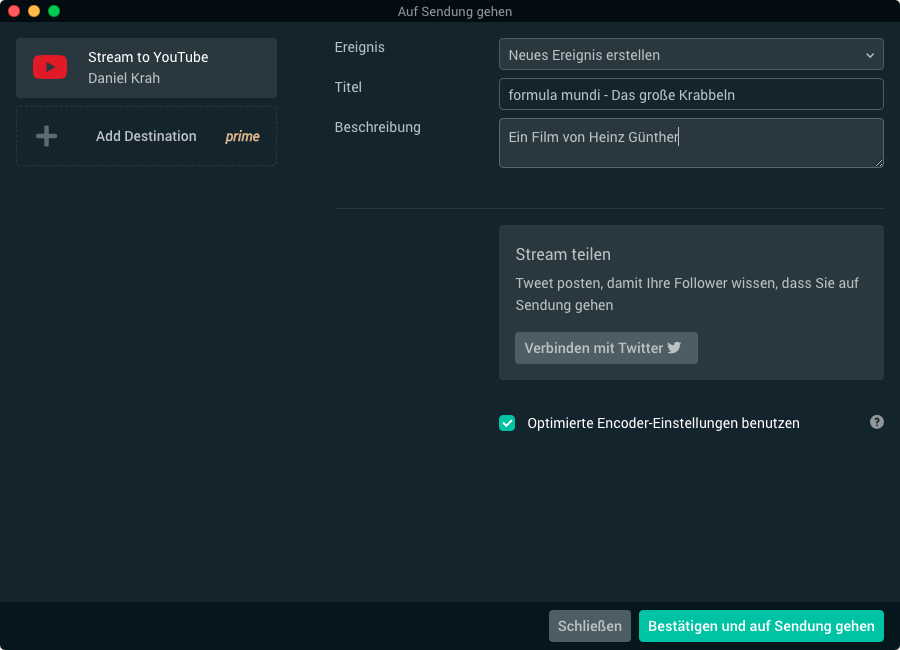
\includegraphics[width=0.9\textwidth]{./pictures/OBSSTUDIO_schnell_aufSendung.png}
\end{center}

% {\vspace{-0.6cm}}
\begin{center}
  \textbf{Vor dem starten des Streams dauert es auch hier etwas.} \\
  {\vspace{0.3cm}}
  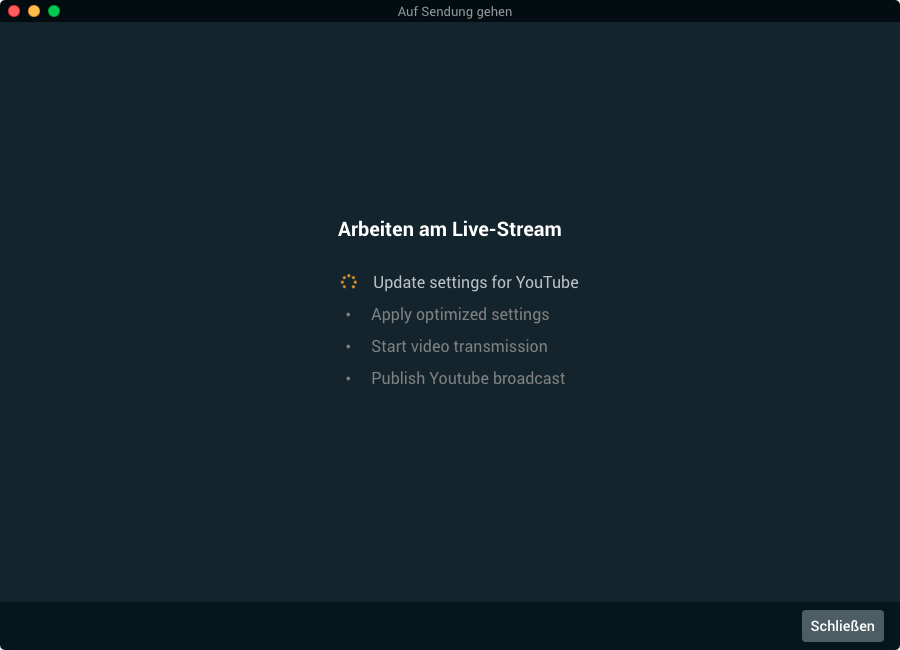
\includegraphics[width=0.7\textwidth]{./pictures/obsStudioIsStartingStream.png}
\end{center}

\newpage
% {\vspace{-0.6cm}}
\begin{center}
  \textbf{Streamlabs OBS hat den Vorteil das es Zugriff auf den Chat hat und man muss nicht den Webbrowser benutzen.} \\
  {\vspace{0.3cm}}
  \includegraphics[width=0.9\textwidth]{./pictures/OBS-STream_Läuft-OBS.png}
\end{center}

% {\vspace{-0.6cm}}
\begin{center}
  \textbf{Hier parallel die Ansicht vom Webbrowser. } \\
  {\vspace{0.3cm}}
  \includegraphics[width=0.9\textwidth]{./pictures/OBS-STream_Läuft-browser.png}
\end{center}



\newpage
% {\vspace{-0.6cm}}
\begin{center}
  \textbf{Natürlich sollte man in den Stream-Einstellungen den Chat konfigurieren} \\
  \textbf{Wichtig sind hierbei die Community-Einstellungen auf welche ich im folgenden Kapitel Youtube Premiere eingehe.} \\
  {\vspace{0.3cm}}
  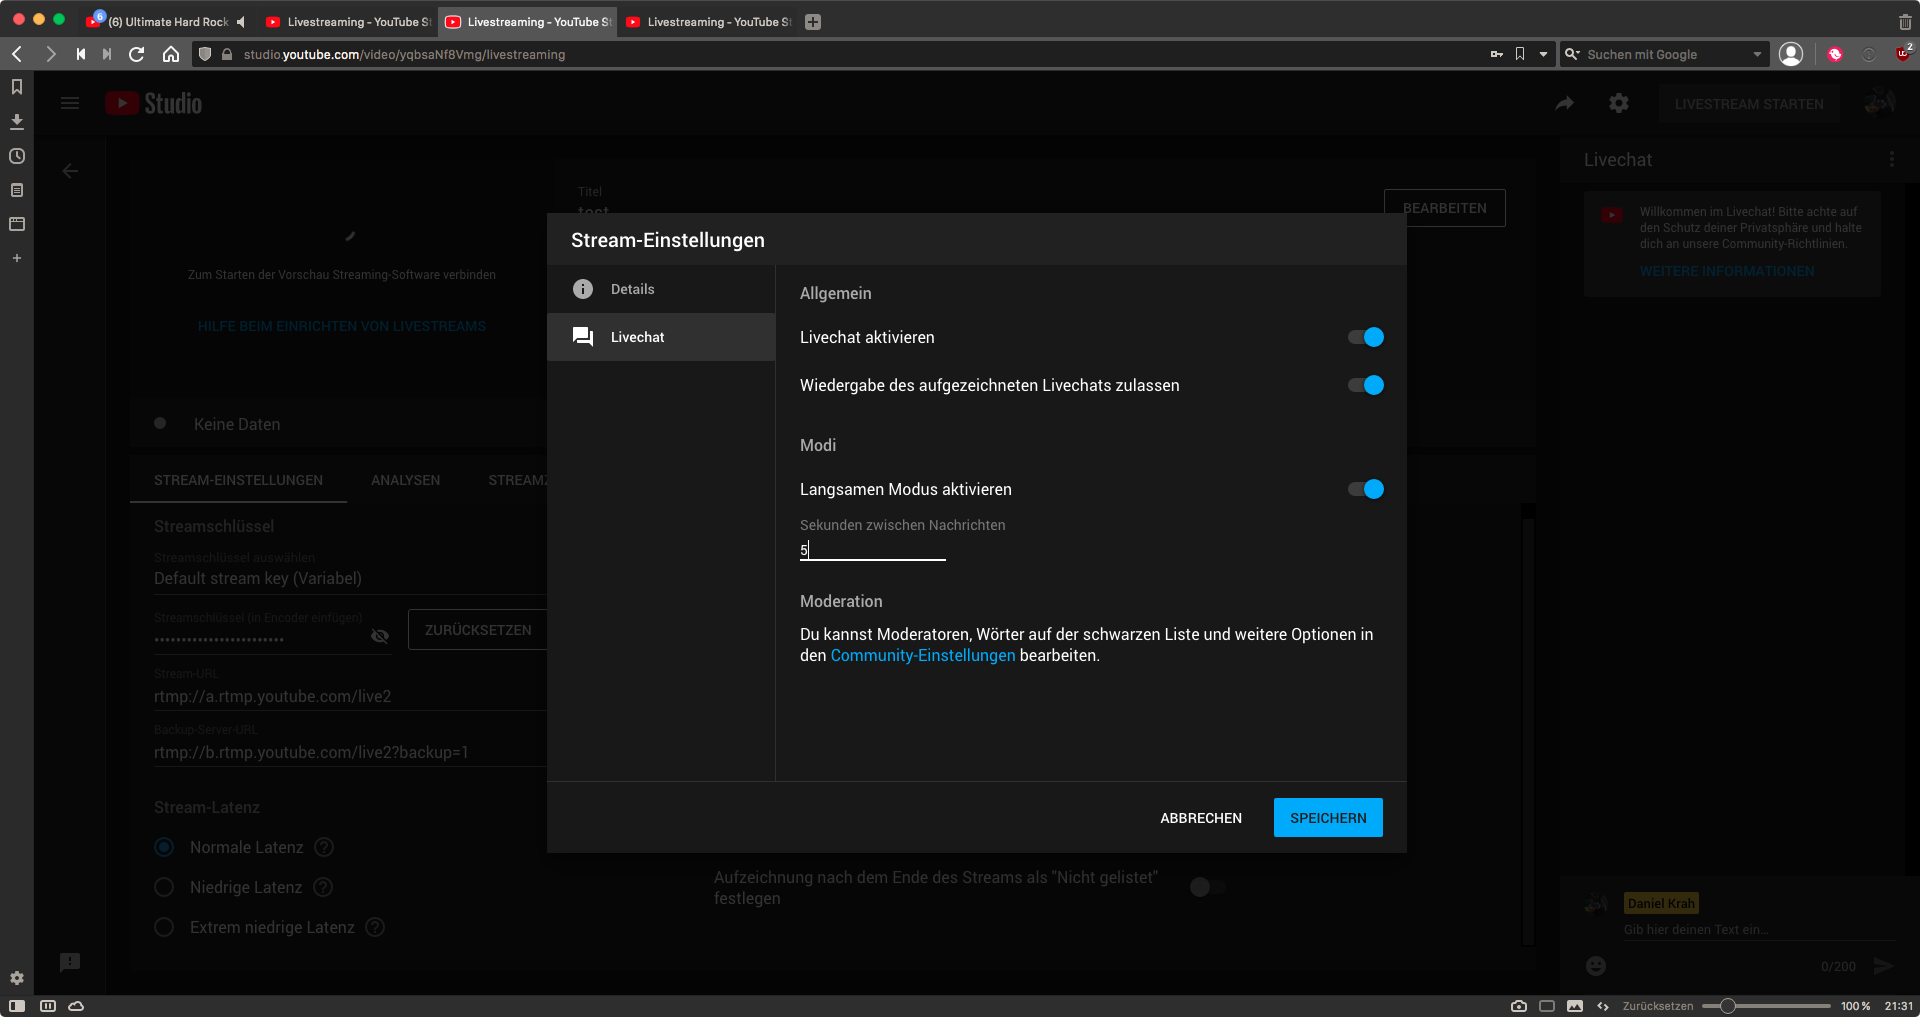
\includegraphics[width=0.9\textwidth]{./pictures/StreamOptionenLivechat.png}
\end{center}
